\documentclass{article}
\usepackage[utf8]{inputenc}
\usepackage{amsmath}
\usepackage{amssymb}
\usepackage{graphicx}

\begin{document}

\section*{Matrix powers}
In this problem we will deal with the problem of computing integer powers of \textbf{square} matrices, defined as
\begin{equation*}
    \mathbf{A}^{k} := \overbrace{\mathbf{A}\cdot \: \dots \: \cdot \mathbf{A}}^{k \text{ times}} \,,\quad k \in \mathbb{N}
\end{equation*}
for $\mathbf{A} \in \mathbb{C}^{n,n}$ and $n \in \mathbb{N}$, $n > 0$.
\subsection*{1-6.a}
We are tasked with implementing a function \verb|matPow| that using only basic algebra operations (including matrix-vector or matrix-matrix multiplications), computes the $k$-th power of the $n \times n$ matrix $\mathbf{
A}$ as efficiently as possible. We are given as input a object of type \verb|Eigen::MatrixXcd| hence a complex entry matrix, all operations from \verb|Eigen::MatrixXd| work here as well. We can import the library \verb|<unsupported/Eigen/MatrixFunctions>| to verify our result using \verb|.pow(k)|. We think back to the lecture Algorithms and data structures here, as we have seen the techniques used there. We employ a divide-and-conquer algorithm. We will demonstrate first how it work for some $k = 2^{m}$ and then also how to make it work for any $k \in \mathbb{N}^{+}$. Given $k = 2^{m}$ we split in each step the product into (where $k = 2l$ for some $l \in \mathbb{N}$)
\begin{equation}
    \mathbf{A}^{k} = \mathbf{A}^{2l} = \mathbf{A}^{l} \cdot \mathbf{A}^{l}
\end{equation}
and applying this recursively gives us the result where the base case is multiplying $\mathbf{A}$ and $\mathbf{A}$ in the usual way. Now if the matrix cannot be multiplied like this because $k$ is not a power of two, then at some point we will have that we will have to deal with a power $\mathbf{A}^{l}$ where $l$ is odd and we can hence not divide by two and compute the result like that. Let us assume that $k=2l + 1$ and hence is odd, we then compute
\begin{equation*}
    \mathbf{A}^{k} = \mathbf{A}^{2l+1} = \mathbf{A}^{l} \cdot \mathbf{A}^{l} \cdot \mathbf{A}
\end{equation*}
hence we can just check if we are in a case where the exponent is odd or even. We will get a recurrence relation given by (the worst case is always getting the odd case, which means an additional matrix multiplication in $\mathcal{O}\left(n^{3}\right)$). We must keep in mind that we will do normally $k$ multiplications and now we do $\mathcal{O}\left(k\right)$ and hence we get $\mathcal{O}\left(n^{3} \cdot \log\left(k\right)\right)$, the corresponding code will be shown on the next page. 

\pagebreak 

\noindent This gives us the following code.

\begin{figure}[!hbt]
    \centering
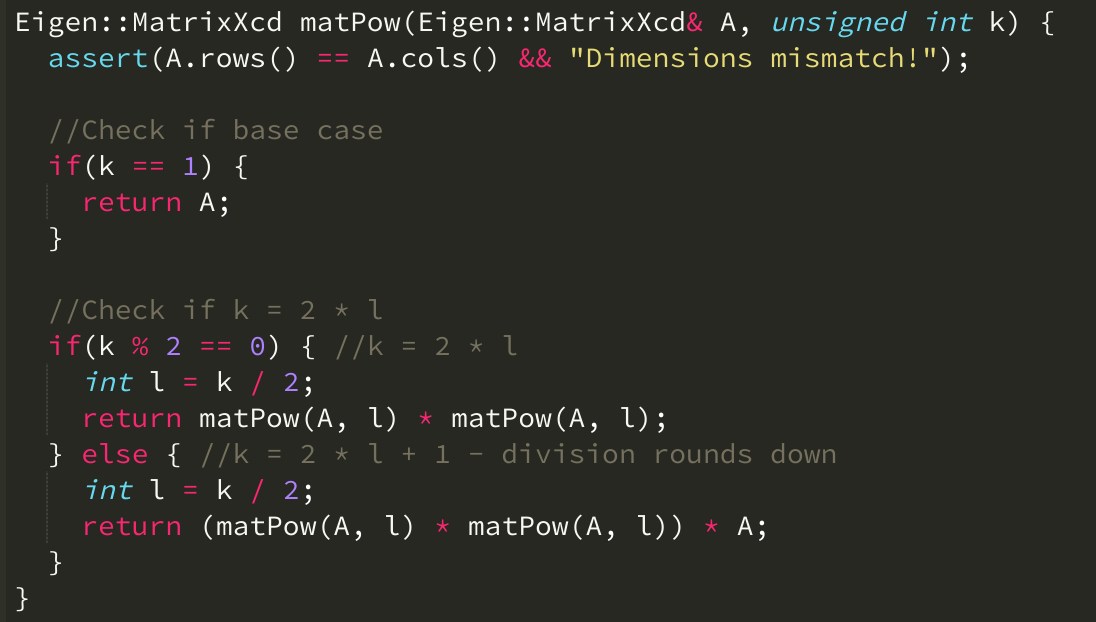
\includegraphics[width=1.0\linewidth]{1-6.a.png}
\end{figure}

\subsection*{1-6.b}
We are asked with computing the asymptotic complexity of our implementation. In the worst case we do $2$ matrix multiplications costing $\mathcal{O}\left(n^{3}\right)$, hence overall with $\left\lceil \log_{2}\right\rceil$ depth to the recursive calls we reach 
\begin{equation*}
    2 \cdot \left\lceil \log_{2}\right\rceil \cdot \mathcal{O}\left(n^{3}\right)
\end{equation*}
\subsection*{1-6.c}
We will skip the part of writing the code that computes the runtime and compares it to the built-in function. We will instead consider what the built-in Eigen library uses.

\subsection*{Matrix Powers in Eigen}

It does not always do what we will discuss here and it also uses a split-based approach, however it can make use of the Schur decomposition, which decomposes a square matrix with complex entries $\mathbf{A}$ into a unitary matrix $\mathbf{Q}$ and an upper triangular matrix $\mathbf{U}$ as
\begin{equation*}
    \mathbf{A} = \mathbf{Q}\mathbf{U}\mathbf{Q}^{-1} = \mathbf{Q}\mathbf{U}\mathbf{Q}^{\mathsf{H}}
\end{equation*}
We now see the following, when taking powers of $\mathbf{A}$ we can use that $\mathbf{Q}\mathbf{Q}^{\mathsf{H}} = \mathbf{Q}^{\mathsf{H}}\mathbf{Q} = \mathbf{I}$, for $\mathbf{A}^{2}$ we get
\begin{equation*}
    \mathbf{A}^{2} = \mathbf{A} \cdot \mathbf{A} = \left(\mathbf{Q}\mathbf{U}\mathbf{Q}^{\mathsf{H}}\right)\cdot\left(\mathbf{Q}\mathbf{U}\mathbf{Q}^{\mathsf{H}}\right) = \mathbf{Q}\mathbf{U}\big(\underbrace{\mathbf{Q}^{\mathsf{H}}\mathbf{Q}}_{= \mathbf{I}}\big)\mathbf{U}\mathbf{Q}^{\mathsf{H}} 
    = \mathbf{Q}\mathbf{U}^{2}\mathbf{Q}^{\mathsf{H}}
\end{equation*}
this does translate to the general case where we get
\begin{equation*}
    \mathbf{A}^{k} = \mathbf{Q}\mathbf{U}^{k}\mathbf{Q}^{\mathsf{H}}
\end{equation*}
We have hence reduced the problem of computing $\mathbf{A}^{k}$ to computing $\mathbf{U}^{k}$. This is however easier, because $\mathbf{U}$ is upper triangular. We will consider to understand why this is the case a somewhat simplified upper triangular $3 \times 3$ matrix given by
\begin{equation*}
    \mathbf{U} = \begin{bmatrix}
    2 & 0 & 2 \\
    0 & 2 & 2 \\
    0 & 0 & 2
    \end{bmatrix}
\end{equation*}
We notice that raising $\mathbf{U}$ to the $k$-th power gives us
\begin{equation*}
     \mathbf{U}^{k} = \begin{bmatrix}
    2 & 0 & 2 \\
    0 & 2 & 2 \\
    0 & 0 & 2
    \end{bmatrix}^{k} = \left(\begin{bmatrix}
    2 & 0 & 0 \\
    0 & 2 & 0 \\
    0 & 0 & 2
\end{bmatrix} + \begin{bmatrix}
    0 & 0 & 2 \\
    0 & 0 & 2 \\
    0 & 0 & 0
   \end{bmatrix}\right)^{k}
\end{equation*}
Powers of diagonal matrices are easy to compute as one can just take the powers of the diagonal elements and the matrix on the right will always evaluate to the zero matrix when taking a power of it. We hence can apply the binomial theorem which also applies to matrices (rings in general, careful that in general the product does not commute, it does here however because the diagonal matrix is equal to $2\cdot \mathbf{I}$)
\begin{align*}
    \left(\begin{bmatrix}
    2 & 0 & 0 \\
    0 & 2 & 0 \\
    0 & 0 & 2
\end{bmatrix} + \begin{bmatrix}
    0 & 0 & 2 \\
    0 & 0 & 2 \\
    0 & 0 & 0
   \end{bmatrix}\right)^{k} = \begin{bmatrix}
    2 & 0 & 0 \\
    0 & 2 & 0 \\
    0 & 0 & 2
\end{bmatrix}^{k} + \binom{k}{1}\begin{bmatrix}
    2 & 0 & 0 \\
    0 & 2 & 0 \\
    0 & 0 & 2
\end{bmatrix}^{k-1} \begin{bmatrix}
    0 & 0 & 2 \\
    0 & 0 & 2 \\
    0 & 0 & 0
   \end{bmatrix}^{1} + \dots \\ \dots+ \binom{k}{k-1}\begin{bmatrix}
    2 & 0 & 0 \\
    0 & 2 & 0 \\
    0 & 0 & 2
\end{bmatrix}^{1} \begin{bmatrix}
    0 & 0 & 2 \\
    0 & 0 & 2 \\
    0 & 0 & 0
   \end{bmatrix}^{k-1} + \begin{bmatrix}
    0 & 0 & 2 \\
    0 & 0 & 2 \\
    0 & 0 & 0
   \end{bmatrix}^{k}
\end{align*}
We now notice that 
\begin{equation*}
    \begin{bmatrix}
    0 & 0 & 2 \\
    0 & 0 & 2 \\
    0 & 0 & 0
   \end{bmatrix}^{i} = \begin{bmatrix}
    0 & 0 & 0 \\
    0 & 0 & 0 \\
    0 & 0 & 0
   \end{bmatrix} \quad \text{if } i > 0
\end{equation*} 
which means that the sum simplifies to 
\begin{align*}
    \left(\begin{bmatrix}
    2 & 0 & 0 \\
    0 & 2 & 0 \\
    0 & 0 & 2
\end{bmatrix} + \begin{bmatrix}
    0 & 0 & 2 \\
    0 & 0 & 2 \\
    0 & 0 & 0
   \end{bmatrix}\right)^{k} &= \begin{bmatrix}
    2 & 0 & 0 \\
    0 & 2 & 0 \\
    0 & 0 & 2
\end{bmatrix}^{k} + \binom{k}{1}\begin{bmatrix}
    2 & 0 & 0 \\
    0 & 2 & 0 \\
    0 & 0 & 2
\end{bmatrix}^{k-1} \begin{bmatrix}
    0 & 0 & 2 \\
    0 & 0 & 2 \\
    0 & 0 & 0
   \end{bmatrix}^{1} \\
   &=\begin{bmatrix}
    2^{k} & 0 & 0 \\
    0 & 2^{k} & 0 \\
    0 & 0 & 2^{k}
\end{bmatrix} + \binom{k}{1}\begin{bmatrix}
    2^{k-1} & 0 & 0 \\
    0 & 2^{k-1} & 0 \\
    0 & 0 & 2^{k-1}
\end{bmatrix}\begin{bmatrix}
    0 & 0 & 2 \\
    0 & 0 & 2 \\
    0 & 0 & 0
   \end{bmatrix} \\
   &=\begin{bmatrix}
    2^{k} & 0 & 0 \\
    0 & 2^{k} & 0 \\
    0 & 0 & 2^{k}
\end{bmatrix} + 2^{k-1}\binom{k}{1}\begin{bmatrix}
    1 & 0 & 0 \\
    0 & 1 & 0 \\
    0 & 0 & 1
\end{bmatrix}\begin{bmatrix}
    0 & 0 & 2 \\
    0 & 0 & 2 \\
    0 & 0 & 0
   \end{bmatrix} 
\end{align*}

\pagebreak

\noindent Continuing where we left off we get

\begin{align*}
    \begin{bmatrix}
    2^{k} & 0 & 0 \\
    0 & 2^{k} & 0 \\
    0 & 0 & 2^{k}
\end{bmatrix} + 2^{k-1}\binom{k}{1}\begin{bmatrix}
    1 & 0 & 0 \\
    0 & 1 & 0 \\
    0 & 0 & 1
\end{bmatrix}\begin{bmatrix}
    0 & 0 & 2 \\
    0 & 0 & 2 \\
    0 & 0 & 0
   \end{bmatrix} &= \begin{bmatrix}
    2^{k} & 0 & 0 \\
    0 & 2^{k} & 0 \\
    0 & 0 & 2^{k}
\end{bmatrix} + 2^{k-1}\binom{k}{1}\begin{bmatrix}
    0 & 0 & 2 \\
    0 & 0 & 2 \\
    0 & 0 & 0
   \end{bmatrix} \\
   &= \begin{bmatrix}
    2^{k} & 0 & 0 \\
    0 & 2^{k} & 0 \\
    0 & 0 & 2^{k}
\end{bmatrix} + \binom{k}{1}\begin{bmatrix}
    0 & 0 & 2^{k} \\
    0 & 0 & 2^{k} \\
    0 & 0 & 0
   \end{bmatrix}
\end{align*}
this reduces the amount of work to do considerably, it of course is not always this easy and the $\mathbf{U}$ matrix does not always contain a zero entry at the position it contains now, but this example was meant to demonstrate how structure can be used to greatly reduce the asymptotic complexity. Now to the task itself the matrix defined by 
\begin{equation*}
    \left(\mathbf{A}\right)_{j,k} := \frac{1}{\sqrt{n}}\text{exp}\left(\frac{2\pi i j k}{n}\right) \,,\quad i,j \in \left\{1, \dots, n\right\}
\end{equation*}
is the scaled Fourier-matrix and is a Vandermonde matrix. The timing is described well in the solutions and they bring little value to understanding the topics, hence they are left out.

\end{document}
